\section{Méthodes d'analyse des signaux}

\subsection{Relation entre centre de pression et centre de masse}

Le centre de pression (CdP) reflète les ajustements actifs du corps pour maintenir son équilibre, tandis que le centre de masse (ou centre de gravité, qui sera appelé CdM) est le point théorique correspondant à la position moyenne de la masse corporelle.
Comprendre la relation entre ces deux notions différentes, bien que corrélées, est essentiel pour comprendre comment et par quels mécanismes le corps maintient son équilibre (dans le cas de l'étude, il est question de l'équilibre orthostatique).
Pour maintenir son équilibre, le corps fait osciller son CdP autour du CdM. 
Le corps ajuste constamment la position du CdP afin que les mouvements du CdM (qui sont présents même dans une position debout immobile) ne sorte de la surface du support (la zone délimitée par le contact des deux pieds au sol). 
Si le CdM sort de cette surface, le corps ne peut plus maintenir son équilibre et une chute est alors possible.
Ces ajustements engagés par le corps montrent alors que l'accélération du CdM est proportionnelle à la différence entre le CdM et le CdP; le CdP entraîne le CdM dans la direction opposée à son déplacement afin de maintenir son équilibre.
Une formule de relation entre le CdP et le CdM a été modélisée à partir de l'équation mécanique simple du pendule inversé (représentant cet entraînement opposé du CdP sur le CdM) : 

\[
    CoP = CoM - \frac{h}{g} \times \frac{d^2 CoM}{dt^2}
\]

Les différentes méthodes d'analyse et leurs modèles mathématiques proposés ci-dessous sont applicables au CdM ou au CdP.
La relation mathématique permettant de passer du CdP au CdM décrite plus tôt est utile pour obtenir des résultats plus précis avec les différentes méthodes décrites dans la suite du rapport.
Ce passage de CdP au CdM est facultative et dépend des habitudes et du niveau de précision demandé par les tests cliniques.

\subsection{Analyse spatio-temporelle}

L'analyse spatio-temporelle permet de déterminer la qualité de l'équilibre orthostatique. 
Elle reflète la capacité du corps d'un patient à maintenir un bon équilibre en position stationnaire droite. 
Le signal étudié est la représentation temporelle de la trajectoire du CdM en position statique debout sur une plateforme statique. 
Il est important de rappeler que ces méthodes sont directement applicables avec le CdP.

\subsubsection{Position moyenne du CdM}

La position moyenne du CdM représente la moyenne de l'ensemble des positions successives du CdM. 
Elle est calculée pour deux types de mouvements : les déplacements médio-latéral ($M_{ml}$), ainsi que pour les déplacements antéro-postérieurs ($M_{ap}$).

\[
M_{AP} = \left( \frac{1}{n} \right) \sum_{n=1}^N \mbox{CoM}_{AP}(n)
\]

\[
M_{ML} = \left( \frac{1}{n} \right) \sum_{n=1}^N \mbox{CoM}_{ML}(n)
\]

Où $CoM$ et la pression du centre de masse suivant la direction AP ou la direction ML.

Plus les valeurs sont basses, plus la qualité de l'équilibre est bonne. 
La position moyenne est régulièrement couplée à l'écart-type, afin de pouvoir les situer l'un par rapport à l'autre, et ainsi donner une idée de la dispersion autour de la moyenne.

\subsubsection{Vitesse moyenne du CdM}

La mesure des longueurs des déplacements du centre de masse sur les deux axes (AP et ML) permettent d'estimer l'énergie dépensée pour la régulation de la posture orthostatique.

\[
L_{AP} = \sum_{n=1}^{N-1} \left| \mbox{CoM}_{AP}(n+1) - \mbox{CoM}_{AP}(n) \right| \tag{5}
\]

\[
L_{ML} = \sum_{n=1}^{N-1} \left| \mbox{CoM}_{ML}(n+1) - \mbox{CoM}_{ML}(n) \right| \tag{6}
\]

\[
MV_{AP} = \frac{L_{AP}}{T}
\]
\[
MV_{AP} = \frac{L_{AP}}{T}
\]

Les vitesses ainsi calculées représentent alors le tracé total en fonction du temps. 
Une vitesse élevée signifie un mauvais équilibre. 
Elles peuvent aussi renseigner sur la consommation d'énergie.

\subsubsection{Valeur quadratique moyenne (RMS pour root mean square)}

\[
RMS_{AP} =\sqrt{  \frac{\sum_{n=1}^{N} \left (\text{CoM}_{AP}(n) \right)^2 }{N}}  \tag{9}
\]

\[
RMS_{ML} =\sqrt{  \frac{\sum_{n=1}^{N} \left (\text{CoM}_{ML}(n) \right)^2 }{N}}  \tag{10}
\]

Le calcul des moyennes quadratiques des amplitudes de déplacement du CdM sur les deux axes définis précédemment permet de quantifier l'habileté à maintenir l'équilibre. 
Plus ces mesures sont basses, plus l'habileté est grande.

\subsubsection{Écart maximal}

\[
R_{AP}= max \left ( \text CoM_{AP} \right ) - min\left ( \text CoM_{AP} \right ) \tag{11}
\]


\[R_{ML}= max \left ( \text CoM_{ML} \right ) - min\left ( \text CoM_{ML} \right ) \tag{12}
\]

L'écart maximal est la différence entre la position maximale et minimale du CdM et est défini suivant les deux axes AP et ML. 
Une augmentation d'une de ces valeurs peut être interprétable en une baisse de la capacité à maintenir l'équilibre postural.

\subsubsection{Surface de l'ellipse de confiance (CEA)}

\[
CEA= 6\pi \sqrt{ \left ( \frac{\sum_{n=1}^{N} \left (\text{CoM}_{AP}(n) \right)^2 \times \sum_{n=1}^{N} \left ( \text{CoM}_{ML}(n) \right)^2}{N^2} \right ) - \left (\frac{\sum_{n=1}^N \text{CoM}_{AP} \times CoM_{ML}}{N} \right)^2} \tag{13}
\]

La surface de l'ellipse de confiance regroupe un certain pourcentage du statokinésigramme (en cm2), ici 95\%. 
Cette intervalle de confiance peut varier selon les pratiques ou les habitudes (certains praticiens utilisent une surface d'ellipse de confiance de 90\% par exemple). 
Plus précisément, c'est l'évolution du périmètre de l'ellipse qui est étudiée. 
Plus ce périmètre est grand, et plus l'équilibre est mauvais.

\begin{figure}[ht]
    \centering
    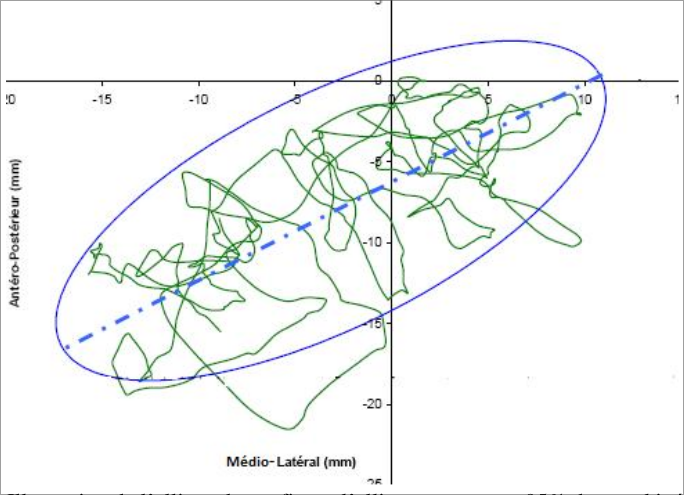
\includegraphics[height=10cm]{images/methode/ellipse_confiance_95.png}
    \caption{Illustration de l'ellipse de confiance (à 95\% du statokinésigramme)}\label{fig:ellipse_confiance}
\end{figure}

\subsubsection{Quotient de Romberg}

\[
QR = \frac{\text{CEA}_{\text{YF}}}{\text{CEA}_{\text{YO}}}\tag{14}
\]

Ce quotient entre la valeur de CEA yeux fermés et la valeur de CEA yeux ouverts permet de mettre en évidence le rôle de la vision dans le contrôle de la posture. 
Une valeur élevée de ce quotient indique une dépendance visuelle accrue dans le maintien de l'équilibre.

\subsection{Analyse spectrale}

L'analyse spectrale se situe dans le domaine fréquentiel. 
Le spectre d'un signal permet d'extraire les différentes composantes présentes dans le signal. 
L'analyse spectrale permet de différencier les différents mécanismes utilisés dans le maintien de l'équilibre en position statique.
Le spectre de fréquence est obtenu en appliquant la transformation de Fourier, principe mathématique, à un signal temporel. 
L'analyse spectrale permet de mettre en évidence l'aspect dynamique du contrôle de la posture orthostatique.

\subsubsection{Fréquence moyenne ou centroïdale}

\[
\text{FM}_{\text{AP}} = \frac{\text{MV}_{\text{AP}}}{4 \cdot \sqrt{2} \cdot \text{M}_{\text{AP}}} \tag{15}
\]

\[
\text{FM}_{\text{ML}} = \frac{\text{MV}_{\text{ML}}}{4 \cdot \sqrt{2} \cdot \text{M}_{\text{ML}}} \tag{16}
\]

La fréquence moyenne est le paramètre qui permet d'étudier le temps nécessaire au mouvement analysé pour revenir dans une position identique. 
Son calcul passe par l'analyse de la distribution fréquentielle des amplitudes.

\subsubsection{Puissance moyenne de la densité spectrale}

La puissance moyenne de la densité spectrale est calculée à partir de l'estimateur de Welch. 
La densité spectrale de puissance permet de mesurer les déplacements du CdP du corps humain.

On part de l'estimation du périodogramme afin de déterminer la densité spectrale de puissance du signal : 

\[
P_{\text{Per}}(f) = \left( \frac{1}{N T_e} \right) \left| \sum_{n=0}^{N-1} x(nT_e)e^{-j2\pi n T_e f} \right|^2
\]

\begin{itemize}
    \item $P_{\text{Per}}(f)$ : C'est le \textbf{périodogramme}, qui est une estimation de la DSP à la fréquence $f$.
    \item $N$ : Nombre d'échantillons du signal.
    \item $T_e$ : Période d'échantillonnage (l'inverse de la fréquence d'échantillonnage, $T_e = \frac{1}{f_e}$, où $f_e$ est la fréquence d'échantillonnage).
    \item $x(nT_e)$ : Valeurs du signal temporel échantillonné à des intervalles $T_e$.
    \item $e^{-j2\pi n T_e f}$ : C'est la base complexe de la transformée de Fourier discrète (TFD) qui décompose le signal en ses composantes fréquentielles.
    \item $\sum_{n=0}^{N-1}$ : La somme sur les échantillons du signal, allant de $n=0$ à $n=N-1$, pour estimer la contribution de chaque fréquence.
    \item $\left| \cdot \right|^2$ : Le carré du module de la transformée de Fourier, qui donne la \textbf{puissance} associée à chaque fréquence.
\end{itemize}

Cette formule est une version discrète du \textbf{périodogramme}, qui permet d'estimer la densité spectrale de puissance d'un signal en fonction de la fréquence $f$. Le processus consiste à :
\begin{itemize}
    \item \textbf{Appliquer la transformée de Fourier discrète (TFD)} au signal $x(nT_e)$ pour transformer le signal temporel en un spectre fréquentiel.
    \item \textbf{Calculer la puissance} à chaque fréquence en prenant le carré du module de la TFD.
    \item \textbf{Normaliser} par $\frac{1}{N T_e}$ pour obtenir une estimation de la DSP, qui représente la distribution de la puissance du signal dans le domaine fréquentiel.
\end{itemize}

Cette estimation permet de voir quelles fréquences contiennent le plus de puissance dans le signal, ce qui est crucial pour l'analyse fréquentielle dans divers domaines, comme la stabilographie, le traitement du signal audio, et d'autres types d'analyse de séries temporelles.

On calcule alors l’estimateur de Welch à partir du périodogramme calculé comme ci-dessus.

\[
P_{Welch}(f) = \frac{1}{L} \sum_{l=1}^{L-1}P_l(f) \tag{18}
\]
\[
P_l(f) = \left( \frac{1}{K}\right) \left |\sum_{n=0}^{K-1} x(n+lK) w(n) e^{-j2\pi nf} \right |^2 \tag{19}
\]

L'estimateur de Welch est une amélioration du périodogramme classique pour estimer la densité spectrale de puissance (DSP) d'un signal. 
Il permet de réduire la variance de l'estimation de la DSP, ce qui en fait une méthode plus robuste pour analyser des signaux bruités ou irréguliers. 
Voici ce que l'estimateur de Welch apporte par rapport au périodogramme simple :

\textbf{1. Réduction de la variance :}
La périodogramme classique a tendance à être un estimateur à variance élevée, c'est-à-dire que ses résultats peuvent fluctuer de manière importante d'un signal à l'autre, même si ceux-ci ont une structure similaire. 
Cela peut rendre l'analyse spectrale moins fiable. 
L'estimateur de Welch réduit cette variance en moyennant plusieurs estimations de la DSP obtenues à partir de segments du signal.

\textbf{2. Segmenter et fenêtrer le signal :}
L'algorithme de Welch divise le signal en plusieurs segments qui se chevauchent partiellement (typiquement de 50\%), et applique une fenêtrage à chaque segment (souvent une fenêtre de Hanning ou de Hamming). 

Ce processus présente plusieurs avantages:
\begin{itemize}
    \item \textbf Segmenter le signal permet de découper le signal en morceaux plus petits, ce qui donne plusieurs petites estimations de la DSP au lieu d'une seule estimation basée sur tout le signal.
    \item \textbf Fenêtrer chaque segment aide à atténuer les discontinuités aux bords des segments, qui pourraient introduire des artefacts dans le domaine fréquentiel, comme des fuites spectrales.
\end{itemize}

\textbf{3. Chevauchement des segments}
Les chevauchements des segments (souvent 50\%) augmentent la quantité d'information utilisée pour chaque estimation locale, améliorant ainsi la stabilité de l'estimation globale. 
Cela permet d'améliorer la résolution fréquentielle tout en conservant une meilleure estimation des puissances.

\textbf{4. Moyenne des DSP :}
Après avoir calculé la transformée de Fourier et le périodogramme pour chaque segment, l'algorithme de Welch prend la moyenne des densités spectrales de puissance (DSP) obtenues. 
Cette moyenne réduit la variance des résultats et améliore la stabilité de l'estimation. 
Le fait de mesurer plusieurs estimations atténue également les fluctuations dues au bruit.

L'estimateur de Welch apporte certains avantages : 
\begin{itemize}
    \item  \textbf{Variance plus fiable} : Comme chaque périodogramme segmenté est moyenné, l'estimateur de Welch a une variance significativement plus fiable que le périodogramme classique, offrant une estimation plus fiable.
    \item \textbf{Meilleure résolution fréquentielle} : Même si chaque segment est plus court que le signal original, l'utilisation du chevauchement permet de conserver une bonne résolution fréquentielle tout en réduisant la variance.
    \item  \textbf{Atténuation des fuites spectrales} : l'application d'une fenêtre sur chaque segment réduit les artefacts induits par les discontinuités aux bords du signal.
\end{itemize}

\begin{figure}[ht]
    \centering
    \begin{subfigure}[b]{0.45\textwidth}
        \centering
        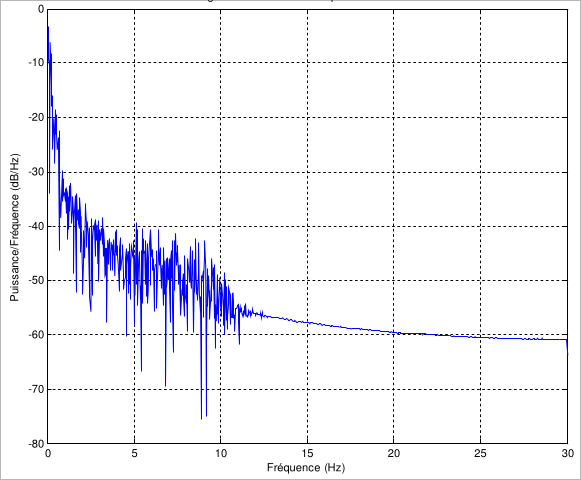
\includegraphics[height=5cm]{images/methode/periodogramme.png}
        \caption{Périodogramme de la densité spectrale de puissance}\label{fig:periodogramme}
    \end{subfigure}
    \begin{subfigure}[b]{0.45\textwidth}
        \centering
        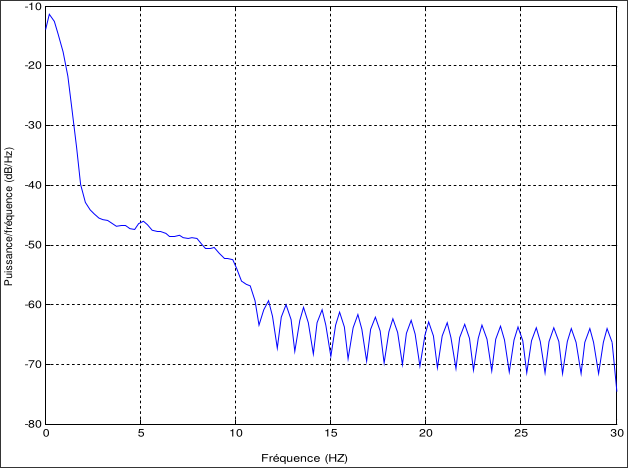
\includegraphics[height=5cm]{images/methode/welch.png}
        \caption{Estimation de Welch de la densité spectrale de puissance}\label{fig:welch}
    \end{subfigure}
    \caption{Comparaison entre le périodogramme et l'estimation de Welch de la densité spectrale de puissance}\label{fig:periodogramme_welch}
\end{figure}


\subsubsection{Pente du spectre de puissance}


Dans le cadre de la stabilographie, l'analyse du spectre dans le 
plan log-log permet de mieux comprendre les mécanismes de régulation
posturale et de quantifier la stabilité ou l'instabilité en 
fonction des fréquences des oscillations du CoP. La régression 
linéaire dans ce contexte permet d'estimer la pente du spectre et 
de révéler les caractéristiques de contrôle postural, avec des 
applications potentielles pour le diagnostic ou la suivi clinique
des troubles de l'équilibre, ou encore pour la prévention des 
chutes chez les personnes âgées.\\


Interprétation en stabilographie : 
\begin{itemize}
\item \textbf Stabilité posturale élevée : 
Lorsque la pente est fortement négative (par exemple au alentour de -2 ou 
plus), cela signifie que la puissance des oscillations posturales 
diminue rapidement avec la fréquence. Dans ce cas, les oscillations 
à basse fréquence dominent, ce qui suggère un contrôle postural 
efficace avec des ajustements lents et stables. Cela pourrait être 
typique chez un jeune adulte en bonne santé.

\item \textbf Instabilité posturale : Lorsque la pente est moins 
négative (par exemple, autour de -1), cela peut signifier que 
les oscillations à haute fréquence contribuent davantage au 
contrôle postural. Ce type de spectre pourrait être observé chez 
des individus plus âgés ou des personnes ayant des troubles de 
l’équilibre, car il indique un contrôle moins stable et une plus 
grande participation des ajustements réflexes ou involontaires.
\end{itemize}


\begin{figure}[H]
    \centering
        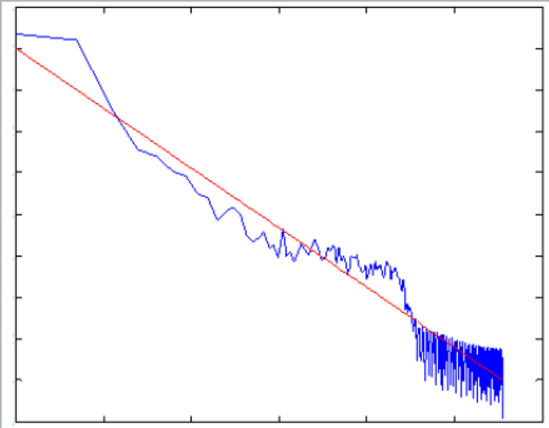
\includegraphics[height=5cm]{images/methode/anaspectrale.png}
        \caption{analyse spectrale et régression linéaire}\label{fig:anaspectrale}
\end{figure}